\author{Carlos Alfredo Cuartas Vélez}
\title{Formación y restauración de imagen en tomografía óptica de coherencia mediante posprocesamiento}

\newcommand\portada{
	\begin{titlepage}
		\begin{center}
			\vfill
			{\large  TESIS DE MAESTRÍA\par}
			{\large Formación y restauración de imagen en tomografía óptica de coherencia mediante posprocesamiento}
			\vfill
			\vfill
			{\large  Carlos Alfredo Cuartas Vélez\\
			ccuarta1@eafit.edu.co \par}
			\vfill
			
			{\normalsize  Escuela de Ciencias \par}
			{\normalsize  Departamento de Ciencias Físicas \par}
			{\normalsize  Maestría en Física Aplicada \par}
			{\normalsize  Universidad EAFIT \par}
			{\normalsize  2017\par}
		\end{center}
	\end{titlepage}
}

\newcommand\contraportada{
	\begin{titlepage}
		\begin{center}
			{\large  FORMACIÓN Y RESTAURACIÓN DE IMAGEN EN TOMOGRAFÍA ÓPTICA DE COHERENCIA MEDIANTE POSPROCESAMIENTO}
			\vfill
			{\large  CARLOS ALFREDO CUARTAS VÉLEZ \par} %Cód 201320001163}
			%{\normalsize ccuarta1@eafit.edu.co}
			\vfill
			{\large  Tesis de Maestría presentada como requerimiento parcial para optar al título de Magíster en Física Aplicada}
			\vfill
			{\large Director \par} 
            {\large Ph.D. RENÉ RESTREPO GÓMEZ \par}
            {\normalsize Universidad EAFIT \par}
            \vfil
            \vspace{18pt}
            {\large  Co-director \par}
            {\large  Ph.D. NÉSTOR URIBE PATARROYO \par}                        
            {\normalsize Wellman Center for Photomedicine, Harvard Medical School and Massachusetts General Hospital \par}
			\vfill
			
			{\normalsize  ESCUELA DE CIENCIAS \par}
			{\normalsize  DEPARTAMENTO DE CIENCIAS FÍSICAS \par}
			{\normalsize  MAESTRÍA EN FÍSICA APLICADA \par}
			{\normalsize  UNIVERSIDAD EAFIT \par}
			{\normalsize  2017\par}
		\end{center}
\end{titlepage}
}

\newcommand \dedicatoria{
	\begin{flushright}
		\vspace*{8cm}
		\emph{``There are not such things as applied sciences,\\ only applications of science''.}\\
		\textbf{Louis Pasteur}\\
		%\emph{``Bajo el ataque de los hombres gamba''}
	\end{flushright}
}

\newcommand \licencia{
\begin{center}
\section*{Licencia}
\end{center}

Este documento se encuentra sujeto a la licencia Reconocimiento-NoComercial-CompartirIgual 2.5 para Colombia de Creative Commons. Para mayor información, visite:
\begin{center}
	\url{https://creativecommons.org/licenses/by-nc-sa/2.5/co/}
\end{center}
\vfill
\begin{center}
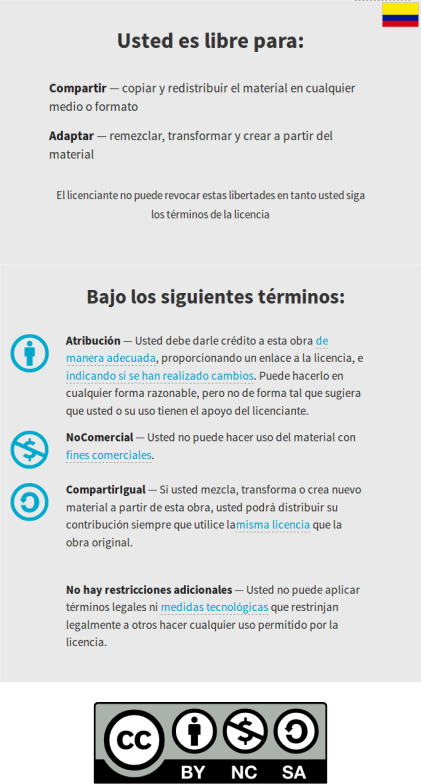
\includegraphics[width=0.65\linewidth]{img/License/licencia}
\end{center}

}

\portada 
\thispagestyle{empty}

\newpage\null\thispagestyle{empty}\newpage

\contraportada
\thispagestyle{empty}
\newpage\null\thispagestyle{empty}\newpage

\thispagestyle{empty}
\newpage

%\begin{abstractpage}\addcontentsline{toc}{chapter}{Abstract}
%	% $Log: abstract.tex,v $
% Revision 1.1  93/05/14  14:56:25  starflt
% Initial revision
%
% Revision 1.1  90/05/04  10:41:01  lwvanels
% Initial revision
%
%
%% The text of your abstract and nothing else (other than comments) goes here.
%% It will be single-spaced and the rest of the text that is supposed to go on
%% the abstract page will be generated by the abstractpage environment.  This
%% file should be \input (not \include 'd) from cover.tex.
La tomografía óptica de coherencia (OCT) es una técnica de imagen médica \textit{no-invasiva} que se basa en interferometría de baja coherencia para producir imágenes con alta resolución axial y lateral de medio inhomogéneos como tejidos. OCT ha visto un alto desarrollo científico y clínico debido a que llena un vacío de resolución existente entre el ultrasonido y la microscopía confocal. La investigación en OCT ha crecido exponencialmente en los últimos años, registrándose alrededor de treinta mil artículos desde su descubrimiento en 1991 hasta el 2015, relacionando las diversas áreas que abarca. Este trabajo está centrado en el entendimiento de los principio básicos y el desarrollo de nuevas técnicas de posprocesamiento para datos provenientes de OCT.

La primera parte del trabajo de grado está orientado a la implementación de los conceptos básicos de OCT para recrear un sistema óptico que permite analizar muestras \textit{ex-vivo}. En el montaje experimental se obtuvo una resolución axial de $\approx2\mu m$ y una resolución lateral de $\approx3 \mu m$, con un escaneo máximo de $\approx1.5mm$ en profundidad y $\approx2.5mm$ de manera lateral, lo que permitió analizar muestras pequeñas. Sin embargo, pese a las regulaciones existentes para el análisis \textit{in-vivo}, el montaje se probó en aplicaciones no médicas de OCT. Las primeras pruebas se realizaron en el escaneo de la topografía de una moneda, en donde se obtuvo una reconstrucción detallada del relieve que esta posee, las mediciones indicaron alturas máximas de $\approx50\mu m$. La segunda muestra que se estudió fue el ala frontal de un insecto \textit{ex-vivo}, donde se pudieron observar estructuras internas tales como la membrana. En este caso, se midió el espesor de la membrana, obteniéndose $\approx5\mu m$.

En la segunda parte del trabajo de grado, se planteó un nuevo método de filtrado de ruido por \speckle a partir del conocimiento de las causas y las características que éste posee, tomando elementos de técnicas de filtrado proveniente de las imágenes de radares de apertura sintética SAR. El algoritmo, conocido como \textit{non-loca means} (\textit{nlmeans}) fue planteado para el caso de ruido blanco, y gracias a sus resultados, ha sido extendido a diversas técnicas de imagen, entre ellas, imágenes SAR, en donde la obtención de los datos hace que también se de la presencia de ruido por \textit{speckle}. Modificando el funcionamiento de \nlmeans en el caso de ruido por \speckle y considerando las características de los datos disponibles en OCT, se propuso una modificación a \nlmeans denotada como \textit{NL-Means-OCT}. En \nlmeansOCT hay una combinación de los conceptos tradicionales de \nlmeans junto con otras implementaciones tridimensionales, lo que convierte a \nlmeansOCT en una herramienta útil para filtrar datos de OCT en donde es necesario la preservación de estructuras finas, o que se encuentran alteradas por la presencia de desplazamientos producidos por el paciente. Los resultados del filtrado con \nlmeansOCT mostraron conservar la fidelidad en la imagen mientras se elimina el ruido por \textit{speckle}. Dadas las características de \nlmeansOCT se pudo implementar de manera satisfactoria en otras áreas en desarrollo de OCT, entre ellas tractografía y gastroenterología.

La última parte del trabajo consistió en el planteamiento de un nuevo método para la corrección de problemas en la fase de un sistema de OCT a partir de fuente de barrido. El problema de la fase surge porque la fuente de barrido tiene fluctuaciones de sincronía con el fotodetector, por lo que la fase del tomograma puede sufrir alteraciones. En vista de que son pocos los algoritmos existentes para abordar este problema, se planteó un método de solución a partir de una optimización, tomando como función objetivo los espectros de potencia asociados con el tomograma, de manera que el espectro de potencia del tomograma afectado se aproxima al de un tomograma ideal mediante una minimización. Aplicando conceptos del enfoque en medios turbios, la implementación muestra encontrar de manera satisfactoria los mapas de corrupción en la fase. Las simulaciones indican que el algoritmo puede encontrar una buena representación del mapa de corrupción real a partir de la aproximación de valores mediante una función de mérito. Los resultados experimentales preliminares verifican la hipótesis de que este modelo mejora los planteamientos actuales de otros autores.


%\end{abstractpage}

\dedicatoria
\newpage\null\thispagestyle{empty}\newpage

\licencia
\addcontentsline{toc}{chapter}{Licencia}
\newpage\null\thispagestyle{empty}\newpage


%\begin{resumen}
%	\addcontentsline{toc}{chapter}{Abstract}
%	% $Log: abstract.tex,v $
% Revision 1.1  93/05/14  14:56:25  starflt
% Initial revision
%
% Revision 1.1  90/05/04  10:41:01  lwvanels
% Initial revision
%
%
%% The text of your abstract and nothing else (other than comments) goes here.
%% It will be single-spaced and the rest of the text that is supposed to go on
%% the abstract page will be generated by the abstractpage environment.  This
%% file should be \input (not \include 'd) from cover.tex.
La tomografía óptica de coherencia (OCT) es una técnica de imagen médica \textit{no-invasiva} que se basa en interferometría de baja coherencia para producir imágenes con alta resolución axial y lateral de medio inhomogéneos como tejidos. OCT ha visto un alto desarrollo científico y clínico debido a que llena un vacío de resolución existente entre el ultrasonido y la microscopía confocal. La investigación en OCT ha crecido exponencialmente en los últimos años, registrándose alrededor de treinta mil artículos desde su descubrimiento en 1991 hasta el 2015, relacionando las diversas áreas que abarca. Este trabajo está centrado en el entendimiento de los principio básicos y el desarrollo de nuevas técnicas de posprocesamiento para datos provenientes de OCT.

La primera parte del trabajo de grado está orientado a la implementación de los conceptos básicos de OCT para recrear un sistema óptico que permite analizar muestras \textit{ex-vivo}. En el montaje experimental se obtuvo una resolución axial de $\approx2\mu m$ y una resolución lateral de $\approx3 \mu m$, con un escaneo máximo de $\approx1.5mm$ en profundidad y $\approx2.5mm$ de manera lateral, lo que permitió analizar muestras pequeñas. Sin embargo, pese a las regulaciones existentes para el análisis \textit{in-vivo}, el montaje se probó en aplicaciones no médicas de OCT. Las primeras pruebas se realizaron en el escaneo de la topografía de una moneda, en donde se obtuvo una reconstrucción detallada del relieve que esta posee, las mediciones indicaron alturas máximas de $\approx50\mu m$. La segunda muestra que se estudió fue el ala frontal de un insecto \textit{ex-vivo}, donde se pudieron observar estructuras internas tales como la membrana. En este caso, se midió el espesor de la membrana, obteniéndose $\approx5\mu m$.

En la segunda parte del trabajo de grado, se planteó un nuevo método de filtrado de ruido por \speckle a partir del conocimiento de las causas y las características que éste posee, tomando elementos de técnicas de filtrado proveniente de las imágenes de radares de apertura sintética SAR. El algoritmo, conocido como \textit{non-loca means} (\textit{nlmeans}) fue planteado para el caso de ruido blanco, y gracias a sus resultados, ha sido extendido a diversas técnicas de imagen, entre ellas, imágenes SAR, en donde la obtención de los datos hace que también se de la presencia de ruido por \textit{speckle}. Modificando el funcionamiento de \nlmeans en el caso de ruido por \speckle y considerando las características de los datos disponibles en OCT, se propuso una modificación a \nlmeans denotada como \textit{NL-Means-OCT}. En \nlmeansOCT hay una combinación de los conceptos tradicionales de \nlmeans junto con otras implementaciones tridimensionales, lo que convierte a \nlmeansOCT en una herramienta útil para filtrar datos de OCT en donde es necesario la preservación de estructuras finas, o que se encuentran alteradas por la presencia de desplazamientos producidos por el paciente. Los resultados del filtrado con \nlmeansOCT mostraron conservar la fidelidad en la imagen mientras se elimina el ruido por \textit{speckle}. Dadas las características de \nlmeansOCT se pudo implementar de manera satisfactoria en otras áreas en desarrollo de OCT, entre ellas tractografía y gastroenterología.

La última parte del trabajo consistió en el planteamiento de un nuevo método para la corrección de problemas en la fase de un sistema de OCT a partir de fuente de barrido. El problema de la fase surge porque la fuente de barrido tiene fluctuaciones de sincronía con el fotodetector, por lo que la fase del tomograma puede sufrir alteraciones. En vista de que son pocos los algoritmos existentes para abordar este problema, se planteó un método de solución a partir de una optimización, tomando como función objetivo los espectros de potencia asociados con el tomograma, de manera que el espectro de potencia del tomograma afectado se aproxima al de un tomograma ideal mediante una minimización. Aplicando conceptos del enfoque en medios turbios, la implementación muestra encontrar de manera satisfactoria los mapas de corrupción en la fase. Las simulaciones indican que el algoritmo puede encontrar una buena representación del mapa de corrupción real a partir de la aproximación de valores mediante una función de mérito. Los resultados experimentales preliminares verifican la hipótesis de que este modelo mejora los planteamientos actuales de otros autores.


%\end{resumen}


\cleardoublepage
\begin{center}
\section*{Agradecimientos}
\end{center}
Quisiera agradecer en primera instancia a mi familia por el apoyo que han dado durante este nuevo capítulo de mi vida. A René y a Néstor por estos años de discusiones, alegatos, frustraciones, asesorías y buenos resultados que hemos obtenido, y que han propiciado un ambiente de trabajo ameno como \textit{compañeros}. A Sebastián por la ayuda con los experimentos. A los compañeros del laboratorio, Camilo con su sentido del humor, Manuela con sus pataletas de niña burgués, y Mateito perrito. A Luciano, por haberme invitado a hacer parte del laboratorio desde hace unos años. Finalmente, a la universidad EAFIT por el apoyo económico mediante los proyectos internos que me permitieron estudiar la Maestría.
\addcontentsline{toc}{chapter}{Agradecimientos}
\newpage\null\thispagestyle{empty}\newpage

\begin{abstract}
	\addcontentsline{toc}{chapter}{Resumen}
	% $Log: abstract.tex,v $
% Revision 1.1  93/05/14  14:56:25  starflt
% Initial revision
%
% Revision 1.1  90/05/04  10:41:01  lwvanels
% Initial revision
%
%
%% The text of your abstract and nothing else (other than comments) goes here.
%% It will be single-spaced and the rest of the text that is supposed to go on
%% the abstract page will be generated by the abstractpage environment.  This
%% file should be \input (not \include 'd) from cover.tex.
La tomografía óptica de coherencia (OCT) es una técnica de imagen médica \textit{no-invasiva} que se basa en interferometría de baja coherencia para producir imágenes con alta resolución axial y lateral de medio inhomogéneos como tejidos. OCT ha visto un alto desarrollo científico y clínico debido a que llena un vacío de resolución existente entre el ultrasonido y la microscopía confocal. La investigación en OCT ha crecido exponencialmente en los últimos años, registrándose alrededor de treinta mil artículos desde su descubrimiento en 1991 hasta el 2015, relacionando las diversas áreas que abarca. Este trabajo está centrado en el entendimiento de los principio básicos y el desarrollo de nuevas técnicas de posprocesamiento para datos provenientes de OCT.

La primera parte del trabajo de grado está orientado a la implementación de los conceptos básicos de OCT para recrear un sistema óptico que permite analizar muestras \textit{ex-vivo}. En el montaje experimental se obtuvo una resolución axial de $\approx2\mu m$ y una resolución lateral de $\approx3 \mu m$, con un escaneo máximo de $\approx1.5mm$ en profundidad y $\approx2.5mm$ de manera lateral, lo que permitió analizar muestras pequeñas. Sin embargo, pese a las regulaciones existentes para el análisis \textit{in-vivo}, el montaje se probó en aplicaciones no médicas de OCT. Las primeras pruebas se realizaron en el escaneo de la topografía de una moneda, en donde se obtuvo una reconstrucción detallada del relieve que esta posee, las mediciones indicaron alturas máximas de $\approx50\mu m$. La segunda muestra que se estudió fue el ala frontal de un insecto \textit{ex-vivo}, donde se pudieron observar estructuras internas tales como la membrana. En este caso, se midió el espesor de la membrana, obteniéndose $\approx5\mu m$.

En la segunda parte del trabajo de grado, se planteó un nuevo método de filtrado de ruido por \speckle a partir del conocimiento de las causas y las características que éste posee, tomando elementos de técnicas de filtrado proveniente de las imágenes de radares de apertura sintética SAR. El algoritmo, conocido como \textit{non-loca means} (\textit{nlmeans}) fue planteado para el caso de ruido blanco, y gracias a sus resultados, ha sido extendido a diversas técnicas de imagen, entre ellas, imágenes SAR, en donde la obtención de los datos hace que también se de la presencia de ruido por \textit{speckle}. Modificando el funcionamiento de \nlmeans en el caso de ruido por \speckle y considerando las características de los datos disponibles en OCT, se propuso una modificación a \nlmeans denotada como \textit{NL-Means-OCT}. En \nlmeansOCT hay una combinación de los conceptos tradicionales de \nlmeans junto con otras implementaciones tridimensionales, lo que convierte a \nlmeansOCT en una herramienta útil para filtrar datos de OCT en donde es necesario la preservación de estructuras finas, o que se encuentran alteradas por la presencia de desplazamientos producidos por el paciente. Los resultados del filtrado con \nlmeansOCT mostraron conservar la fidelidad en la imagen mientras se elimina el ruido por \textit{speckle}. Dadas las características de \nlmeansOCT se pudo implementar de manera satisfactoria en otras áreas en desarrollo de OCT, entre ellas tractografía y gastroenterología.

La última parte del trabajo consistió en el planteamiento de un nuevo método para la corrección de problemas en la fase de un sistema de OCT a partir de fuente de barrido. El problema de la fase surge porque la fuente de barrido tiene fluctuaciones de sincronía con el fotodetector, por lo que la fase del tomograma puede sufrir alteraciones. En vista de que son pocos los algoritmos existentes para abordar este problema, se planteó un método de solución a partir de una optimización, tomando como función objetivo los espectros de potencia asociados con el tomograma, de manera que el espectro de potencia del tomograma afectado se aproxima al de un tomograma ideal mediante una minimización. Aplicando conceptos del enfoque en medios turbios, la implementación muestra encontrar de manera satisfactoria los mapas de corrupción en la fase. Las simulaciones indican que el algoritmo puede encontrar una buena representación del mapa de corrupción real a partir de la aproximación de valores mediante una función de mérito. Los resultados experimentales preliminares verifican la hipótesis de que este modelo mejora los planteamientos actuales de otros autores.


	%\newpage\null\thispagestyle{empty}\newpage
\end{abstract}
